\documentclass[11pt,a4paper]{article}

\usepackage[margin=2cm,top=2.2cm,bottom=2.2cm]{geometry}
\usepackage{graphicx}
\usepackage{adjustbox}
\usepackage{titlesec}
\usepackage{enumitem}
\usepackage{hyperref}
\usepackage{fancyhdr}
\usepackage{xcolor}
\usepackage{setspace}
\usepackage{helvet}
\usepackage[T1]{fontenc}
\usepackage{tikz}
\usepackage{float}
\usepackage{placeins}
\usepackage{pdflscape}
\usepackage{caption}

\setlength{\parskip}{0.45em plus 0.1em minus 0.05em}
\setlength{\parindent}{0pt}
\captionsetup{font=small, labelfont=bf, skip=6pt}
\floatplacement{figure}{htbp}

\renewcommand{\familydefault}{\sfdefault}

\definecolor{brandblue}{HTML}{1e3a8a}
\definecolor{brandlight}{HTML}{dbeafe}
\definecolor{textgray}{HTML}{475569}

\hypersetup{
    colorlinks=true,
    linkcolor=brandblue,
    urlcolor=brandblue,
    pdftitle={AI-Based HSRP Operations and Analytics Framework},
    pdfauthor={Real Industries Limited}
}

\pagestyle{fancy}
\fancyhf{}
\fancyhead[L]{\small\textcolor{textgray}{Real Mazon --- HSRP Operations}}
\fancyhead[R]{\small\textcolor{textgray}{Real Industries Limited}}
\fancyfoot[C]{\small\textcolor{textgray}{\thepage}}
\renewcommand{\headrulewidth}{0.4pt}
\renewcommand{\footrulewidth}{0pt}

\titleformat{\section}{\Large\bfseries\color{brandblue}}{}{0em}{}[\titlerule]
\titleformat{\subsection}{\large\bfseries\color{brandblue}}{}{0em}{}
\titlespacing*{\section}{0pt}{1em}{0.5em}
\titlespacing*{\subsection}{0pt}{0.8em}{0.35em}

\newcommand{\capblock}[3]{%
    \vspace{0.25em}
    \noindent\textbf{#1}\\[0.15em]
    #2
    \vspace{0.2em}
    \noindent\textit{Business value:} #3
    \vspace{0.35em}
}

% Scaled figure helper — fits page without float gaps
\newcommand{\docfig}[5]{%
    \begin{figure}[#1]
        \centering
        \adjustbox{max width=\textwidth, max height=#2, center}{%
            \includegraphics{#3}%
        }%
        \caption{#4}
        \label{#5}
    \end{figure}%
}

% --- Cover page ---
\newcommand{\makecover}{%
    \thispagestyle{empty}
    \begin{center}
        \vspace*{1.5cm}
        {\color{brandblue}\rule{\textwidth}{2pt}}\\[0.8cm]
        {\fontsize{28}{34}\selectfont\bfseries\color{brandblue} Real Mazon}\\[0.3cm]
        {\large The Vehicle Identification Company}\\[1.2cm]
        {\fontsize{22}{28}\selectfont\bfseries AI-Based HSRP Operations}\\[0.2cm]
        {\fontsize{22}{28}\selectfont\bfseries \& Analytics Framework}\\[1.5cm]
        {\Large Real Industries Limited}\\[0.4cm]
        {\large PAN India High Security Registration Plate Operations}\\[2cm]
        
\begin{tikzpicture}
            \fill[brandlight, rounded corners=4pt] (0,0) rectangle (10,1.2);
            \node at (5,0.6) {\textbf{\color{brandblue} Confidential --- For Management Review}};
        \end{tikzpicture}\\[2cm]
        {\large \today}\\[0.5cm]
        {\color{textgray} Proposed Vision Document}
        \vfill
        {\color{brandblue}\rule{\textwidth}{2pt}}
    \end{center}
    \newpage
}

\begin{document}

\makecover

\tableofcontents
\newpage

% =============================================================================
\section{Executive Summary}

Real Industries Limited, operating under the brand \textbf{Real Mazon}, is one of India's leading manufacturers and suppliers of High Security Registration Plates (HSRP). As operations expand across states, OEMs, embossing stations, and fitment centers, management needs a single, intelligent view of the entire HSRP lifecycle.

This document proposes an \textbf{AI-powered operations and analytics framework} that brings together data from OEM portals, embossing stations (ESOs), warehouses, dealers, and fitment centers into one national operations platform.

\textbf{What management will gain:}
\begin{itemize}[leftmargin=1.5em, itemsep=0.3em]
    \item Real-time visibility into orders, revenue, and pendency across all of India
    \item Intelligent alerts that predict delays, stock shortages, and performance issues before they escalate
    \item Executive dashboards and downloadable MIS reports for faster, data-driven decisions
    \item End-to-end tracking from order receipt through issuance, embossing, dispatch, and fitment
    \item An \textbf{LLM-powered AI assistant} for natural-language operational queries and an \textbf{ML prediction layer} for revenue, pendency, and inventory forecasting
\end{itemize}

The framework positions Real Industries Limited to operate as a fully data-driven, predictive HSRP enterprise --- strengthening service to OEMs, transport departments, and dealers nationwide.

% =============================================================================
\section{About Real Industries Limited}

Real Industries Limited has emerged as a trusted national partner in the manufacturing, issuance, and distribution of High Security Registration Plates. Through advanced production infrastructure, compliance-driven operations, and robust quality control, the company serves authorized dealers and major automobile OEMs across India.

By ensuring secure, authenticated, and traceable issuance of registration plates, Real Industries plays a vital role in:
\begin{itemize}[leftmargin=1.5em, itemsep=0.2em]
    \item Strengthening national transport security
    \item Preventing vehicle-related crimes through tamper-proof identification
    \item Supporting transparent vehicle identification systems nationwide
\end{itemize}

Operating at PAN India scale requires more than manufacturing excellence --- it requires \textbf{operational intelligence} that connects every stakeholder in the HSRP value chain.

% =============================================================================
\section{Business Challenge}

Today, HSRP operations generate vast amounts of data across multiple channels --- but this information often remains fragmented:

\begin{itemize}[leftmargin=1.5em, itemsep=0.3em]
    \item \textbf{OEM portals} (DISHA, Hero Biz, Old Vehicle Portal, POS) receive orders independently
    \item \textbf{Embossing stations (ESOs)} process plates with varying productivity and rejection rates
    \item \textbf{Warehouses} hold stock that must be balanced across states and OEMs
    \item \textbf{Dealers and fitment centers} complete the final stage of plate installation
\end{itemize}

Without a unified view, management faces delayed visibility into revenue trends, operational bottlenecks, inventory risks, and service-level breaches. Critical decisions --- such as stock replenishment, ESO workload balancing, and OEM relationship management --- rely on manual reporting rather than live intelligence.

% =============================================================================
\section{Proposed Solution Overview}

The proposed \textbf{AI-Powered HSRP Operations \& Analytics Ecosystem} provides centralized, real-time visibility into the complete HSRP lifecycle --- from order receipt to embossing, dispatch, inventory management, fitment, and performance monitoring across India.

The system integrates data from all operational touchpoints to create a \textbf{unified national operations dashboard}. An AI intelligence layer continuously analyses this data to generate forecasts, detect anomalies, and recommend corrective actions --- while management retains full oversight through escalation workflows for critical exceptions.

The following sections present the architecture (Figure~\ref{fig:architecture}), platform technology stack (Figure~\ref{fig:platform}), order lifecycle (Figure~\ref{fig:lifecycle}), and PAN India ecosystem (Figure~\ref{fig:ecosystem}).

% =============================================================================
\section{Architecture Overview}

The architecture flows through eight interconnected stages, from data input to measurable business outcomes:

\begin{enumerate}[leftmargin=1.5em, itemsep=0.4em]
    \item \textbf{Input Sources} --- Orders and operational data from OEM portals, ESOs, warehouses, dealers, and fitment centers
    \item \textbf{Data Unification} --- Central collection, validation, and classification of New and Old vehicle orders
    \item \textbf{AI Decision Engine} --- ML prediction models (revenue, pendency, stock, TAT), automated rule engine, feature store, and model orchestration
    \item \textbf{Management Review} --- Straight-through processing for low-risk insights; human escalation for critical pendency, SLA breaches, and stock risks
    \item \textbf{Core HSRP Workflow} --- Issuance, embossing, dispatch, fitment, and automated customer/OEM notifications
    \item \textbf{Enterprise Integration} --- OEM portal APIs, dealer systems, transport reporting, notification services, and secure API gateway
    \item \textbf{Analytics \& Governance} --- Live KPI dashboards, model monitoring, MIS exports, audit trails, and role-based access control
    \item \textbf{Business Outcomes} --- Faster decisions, reduced delays, optimized inventory, and improved service levels
\end{enumerate}

A secure data foundation supports the entire platform, with a continuous feedback loop that refines ML models through performance feedback and new order data.

\begin{landscape}
\thispagestyle{fancy}
\begin{figure}[p]
    \vspace*{-0.8cm}
    \centering
    \adjustbox{max width=\linewidth, max height=0.76\paperheight, center}{%
        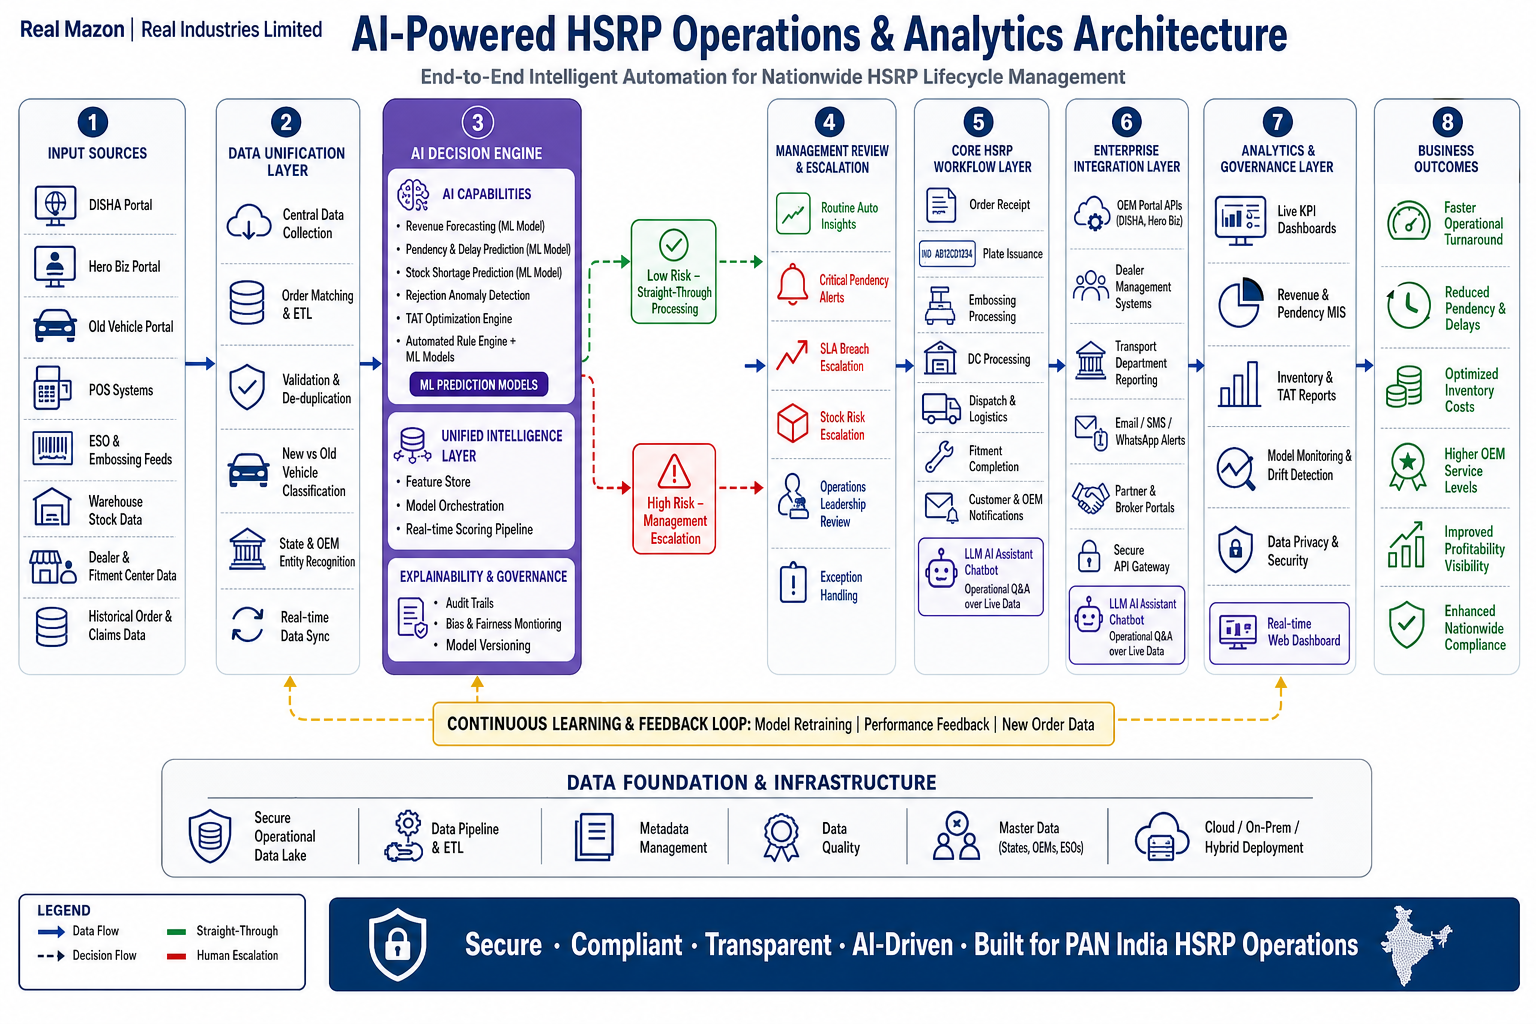
\includegraphics{images/hsrp-architecture-flow.png}%
    }
    \caption{AI-Powered HSRP Operations \& Analytics Architecture --- end-to-end intelligent operations for nationwide HSRP lifecycle management.}
    \label{fig:architecture}
    \vspace*{-0.4cm}
\end{figure}
\end{landscape}

\FloatBarrier
% =============================================================================
\section{Platform \& AI Technology}

Beyond business dashboards, the platform includes a focused AI and technology stack designed for PAN India HSRP scale (Figure~\ref{fig:platform}).

\docfig{htbp}{0.46\textheight}{images/hsrp-platform-architecture.png}{Real Mazon HSRP platform architecture --- technology layers from presentation to data foundation.}{fig:platform}

\subsection{ML Prediction Models}

Machine learning models analyse historical order, revenue, inventory, and performance data to generate forward-looking intelligence:
\begin{itemize}[leftmargin=1.5em, itemsep=0.25em]
    \item \textbf{Revenue forecasting} --- state, OEM, and portal-wise revenue trend prediction
    \item \textbf{Pendency \& delay prediction} --- early warning of stage bottlenecks and SLA breach risk
    \item \textbf{Stock shortage prediction} --- 7-day inventory risk alerts by warehouse and OEM
    \item \textbf{TAT forecasting} --- expected turnaround time by state, ESO, and lifecycle stage
    \item \textbf{Workload prediction} --- embossing station capacity and order volume planning
\end{itemize}

Models are supported by a \textbf{feature store}, \textbf{real-time scoring pipeline}, and \textbf{model versioning} for continuous improvement.

\subsection{LLM AI Assistant Chatbot}

An \textbf{LLM-powered operations assistant} (Azure OpenAI) enables management and operations teams to ask natural-language questions over live HSRP data --- for example, ``Which states have the highest pendency this week?'' or ``Forecast next month's order volume for new vehicles.''

The assistant uses a \textbf{LangChain agent} connected to live analytics tools covering revenue, pendency, inventory, ESO performance, TAT, and forecasting --- providing instant answers without manual report generation.

\subsection{Automated Rule Engine \& Smart Alerts}

A background \textbf{rule engine} runs on a scheduled cycle (every 15 minutes) to evaluate SLA thresholds, stock levels, rejection spikes, and pendency limits. Critical findings trigger \textbf{smart alerts}; optional AI enrichment adds context and recommended actions for management review.

\subsection{Integration \& Real-Time Layer}

\begin{itemize}[leftmargin=1.5em, itemsep=0.25em]
    \item \textbf{REST API gateway} --- secure access for dashboards, reports, and partner integrations
    \item \textbf{OEM portal connectors} --- automated sync from DISHA, Hero Biz, Old Vehicle Portal, and POS
    \item \textbf{WebSocket live updates} --- real-time order and monitoring data to the operations console
    \item \textbf{JWT authentication} --- role-based secure access for management users
    \item \textbf{Scheduled jobs} --- automated alert generation and portal data synchronization
\end{itemize}

\subsection{Data Foundation}

All layers rest on a secure \textbf{operational data store} (PostgreSQL in production, with development support), \textbf{master data management} for states, OEMs, ESOs, and dealers, plus \textbf{audit logging} and \textbf{data quality} controls. The platform supports \textbf{cloud, on-premise, or hybrid} deployment.

% =============================================================================
\section{HSRP Order Lifecycle}

Every HSRP order progresses through defined stages: \textbf{Order Received} $\rightarrow$ \textbf{Issuance Pending} $\rightarrow$ \textbf{Embossing Pending} $\rightarrow$ \textbf{DC Pending} $\rightarrow$ \textbf{Dispatch Pending} $\rightarrow$ \textbf{Fitment Pending} $\rightarrow$ \textbf{Completed}.

New vehicle orders are typically OEM-led, flowing from manufacturer portals through embossing to dealer fitment. Old vehicle orders follow a dealer and fitment-center-led path. The proposed system monitors turnaround time and delays at every stage, for every state and ESO (Figure~\ref{fig:lifecycle}).

\docfig{htbp}{0.3\textheight}{images/hsrp-order-lifecycle.png}{HSRP order lifecycle from receipt to completed fitment, applicable to both New and Old vehicles.}{fig:lifecycle}

\FloatBarrier
% =============================================================================
\section{PAN India Ecosystem}

The National Operations Center serves as the intelligence hub, receiving data from all regional and partner touchpoints and returning actionable insights to operations leadership (Figure~\ref{fig:ecosystem}).

\docfig{htbp}{0.52\textheight}{images/hsrp-ecosystem-map.png}{PAN India HSRP ecosystem --- the National Operations Center connects states, OEMs, ESOs, warehouses, fitment centers, portals, and dealers.}{fig:ecosystem}

% =============================================================================
\section{Capability Modules}

The framework comprises eight integrated capability modules. Each module is designed to answer specific management questions and drive measurable business outcomes.

% --- Module 1 ---
\subsection{Revenue \& OEM Analytics}

\capblock{Purpose}{%
Track how revenue and order volumes are distributed across states, OEMs, and source portals --- for both New and Old vehicles. Management can view daily, weekly, and monthly trends, compare OEM performance, and analyse portal-wise contribution from DISHA, Hero Biz, Old Vehicle Portal, and POS systems.}{%
Identify high-performing OEMs and states, detect low-revenue regions requiring intervention, forecast future revenue trends, and enable strategic management decisions. Downloadable reports and executive presentation exports support board-level reviews.}

% --- Module 2 ---
\subsection{Pendency \& Delay Monitoring}

\capblock{Purpose}{%
Monitor where orders are stuck across the lifecycle --- by state, OEM, and ESO. Stage-wise bottleneck analysis covers Issuance Pending, Embossing Pending, DC Pending, and Fitment Pending for both New and Old vehicles.}{%
Auto-detect operational bottlenecks, predict delays before they become critical, trigger escalation for SLA breaches, and recommend real-time operational interventions. Consolidated dashboards and exception-based alerts ensure leadership focuses on what matters most.}

% --- Module 3 ---
\subsection{Operational Performance Analytics}

\capblock{Purpose}{%
Measure how effectively embossing stations, dealers, and fitment centers are performing. Track monthly ESO productivity, rejection rates, order frequency by state and OEM, and PAN India active counts for OEMs, dealers, and ESOs.}{%
Identify underperforming ESOs, predict operational workload, detect abnormal rejection spikes, and recommend process improvements. Automated management summaries reduce time spent on manual performance reporting.}

% --- Module 4 ---
\subsection{Inventory \& Consumption Intelligence}

\capblock{Purpose}{%
Provide real-time visibility into stock levels across warehouses, broken down by OEM, state, plate size, and colour. Analyse consumption patterns and compare historical trends.}{%
Predict stock shortages in advance, recommend inter-state stock balancing, auto-generate replenishment alerts, and prevent both overstocking and understocking. AI-driven procurement planning supports manufacturing and warehouse teams.}

% --- Module 5 ---
\subsection{AI Smart Alerts \& Predictive Intelligence}

\capblock{Purpose}{%
The AI engine combines \textbf{ML prediction models} and an \textbf{automated rule engine} to generate intelligent alerts --- stock shortage forecasts (7-day horizon), underperforming ESO identification, monthly order volume predictions, dispatch delay warnings, and abnormal rejection detection. Alerts can be enriched with AI-generated context and recommended actions.}{%
Enable proactive management rather than reactive firefighting. Automated exception alerts ensure critical issues reach the right decision-makers without manual monitoring.}

% --- Module 6 ---
\subsection{Real-Time Dashboard \& Monitoring}

\capblock{Purpose}{%
Live operational dashboards for New and Old vehicle orders, with state-wise tracking, ESO workload visibility, embossing station monitoring, dispatch status, and dealer/fitment center activity. Interactive visual analytics with geo-based heatmaps and \textbf{WebSocket real-time updates} provide at-a-glance national situational awareness. The integrated \textbf{LLM AI assistant} allows managers to query live data in natural language.}{%
Executive management gains instant visibility into nationwide operations from any device. Drill-down intelligence and conversational AI support allow regional teams to investigate issues without waiting for scheduled reports.}

% --- Module 7 ---
\subsection{TAT (Turnaround Time) Analysis}

\capblock{Purpose}{%
Measure how long each lifecycle stage takes --- from order to issuance, issuance to embossing, embossing to dispatch, and dispatch to fitment. Benchmark average TAT by state, OEM, and ESO with delay trend analysis.}{%
Predict future TAT performance, identify root causes of delays, and recommend operational optimizations. Stage-wise efficiency benchmarking drives continuous improvement across the network.}

% --- Module 8 ---
\subsection{Predictive Inventory Planning}

\capblock{Purpose}{%
Forecast future inventory needs based on seasonal patterns, festival demand, state-specific consumption, and OEM-specific requirements. Generate minimum stock alerts and automated replenishment recommendations.}{%
Reduce inventory holding costs, ensure uninterrupted HSRP supply, improve warehouse efficiency, and optimize manufacturing planning aligned with predicted demand.}

% =============================================================================
\section{Strategic Benefits}

The proposed AI-powered HSRP ecosystem will significantly enhance operational efficiency and management visibility across India:

\begin{itemize}[leftmargin=1.5em, itemsep=0.35em]
    \item \textbf{Real-time operational visibility} across all states, OEMs, and ESOs
    \item \textbf{Automated MIS and reporting} --- reducing manual effort and reporting delays
    \item \textbf{Smart delay and rejection monitoring} with predictive escalation
    \item \textbf{Predictive operational intelligence} for inventory, revenue, and workload planning
    \item \textbf{Performance optimization} through data-driven process improvements
    \item \textbf{Faster decision-making} at every level of operations leadership
    \item \textbf{Improved inventory planning} that prevents supply disruptions
    \item \textbf{Reduced operational bottlenecks} through early detection and intervention
    \item \textbf{Enhanced customer and OEM service levels} through proactive management
    \item \textbf{Nationwide centralized monitoring} from a single operations platform
\end{itemize}

% =============================================================================
\section{Conclusion}

The proposed \textbf{AI-Based HSRP Operations \& Analytics Framework} will transform Real Industries Limited into a fully data-driven, intelligent, and predictive HSRP operations enterprise.

By integrating AI, analytics, real-time dashboards, and predictive intelligence into manufacturing, issuance, embossing, dispatch, inventory, and fitment operations, the company can achieve higher operational efficiency, stronger compliance monitoring, optimized resource utilization, and superior nationwide service delivery.

This framework will position Real Industries Limited --- and the Real Mazon brand --- as one of India's most technologically advanced and operationally intelligent HSRP solution providers.

\vspace{1.5em}
\begin{center}
    {\color{brandblue}\rule{0.6\textwidth}{1.5pt}}\\[0.5em]
    \textit{Secure \textperiodcentered\ Compliant \textperiodcentered\ Transparent \textperiodcentered\ AI-Driven}\\[0.3em]
    \textbf{\color{brandblue}Built for PAN India HSRP Operations}
\end{center}

\end{document}
